\section{Saving}\label{saving}

Every time users leave a sketch, Foldlings archives the sketch to a
file, which can then be restored. Users restore a sketch by tapping on
one of the cards on the main screen. These cards can be deleted through
a long press on the sketch, which presents an option to remove the saved
file. This convention is familiar to iOS users.

\begin{figure}[htbp]
\centering
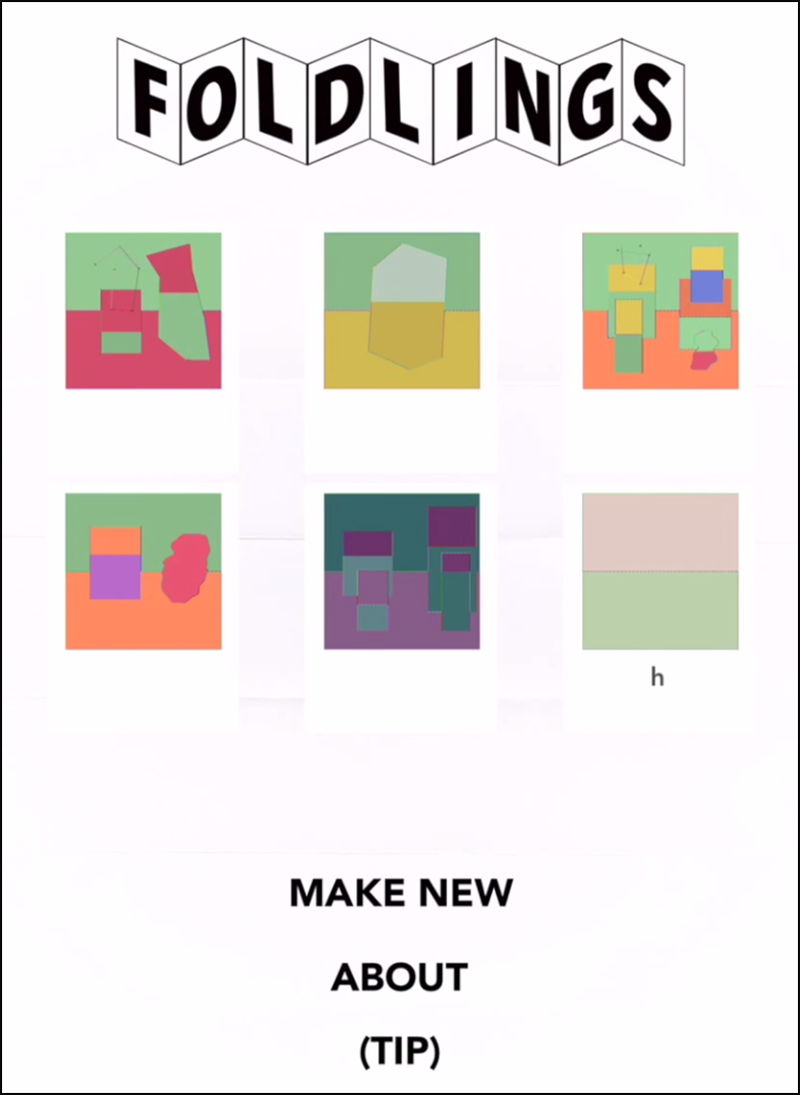
\includegraphics{figures/34_UI_Saving/saved_sketches.png}
\caption{Saved sketches displayed on the main screen.}
\end{figure}

In addition, we also save fold patterns for user designs to Amazon S3.
Saving these files allows us to debug user problems remotely and see the
kinds of cards users attempt to make with our software. Along with user
testing, these captured sketches have been instrumental to our design
process.
